\documentclass[border=2pt]{standalone}
% Shared preamble for the standalone result plots (fig/src/*.tex).
% Compile:  tectonic -X compile fig/src/<name>.tex --outdir fig/src/out
% then copy fig/src/out/<name>.pdf over fig/<name>.pdf
%
% Palette matches the paper: wacvblue is main.tex's link colour, orange is xcolor's.
\usepackage{iftex}
\ifXeTeX
  \usepackage{fontspec}
  \setmainfont{texgyretermes}[Extension=.otf, UprightFont=*-regular,
    BoldFont=*-bold, ItalicFont=*-italic, BoldItalicFont=*-bolditalic]
\fi
\usepackage{pgfplots}
\pgfplotsset{compat=1.18}
\usepackage{amsmath}
\definecolor{wacvblue}{rgb}{0.21,0.49,0.74}
\pgfplotsset{
  resultaxis/.style={
    axis background/.style={fill=white},
    grid=major, ymajorgrids=true, xmajorgrids=false,
    grid style={gray!25, line width=0.3pt},
    tick align=outside, tick pos=left,
    label style={font=\small}, tick label style={font=\small},
    legend style={font=\small, draw=gray!50, fill=white, fill opacity=0.9,
                  text opacity=1, inner sep=2pt},
  },
  vidmark/.style={wacvblue, mark=*, thick, mark size=2.2pt},
  eegmark/.style={orange, mark=o, thick, dashed, mark size=2.2pt},
}

\definecolor{hired}{RGB}{191,0,0}
\begin{document}
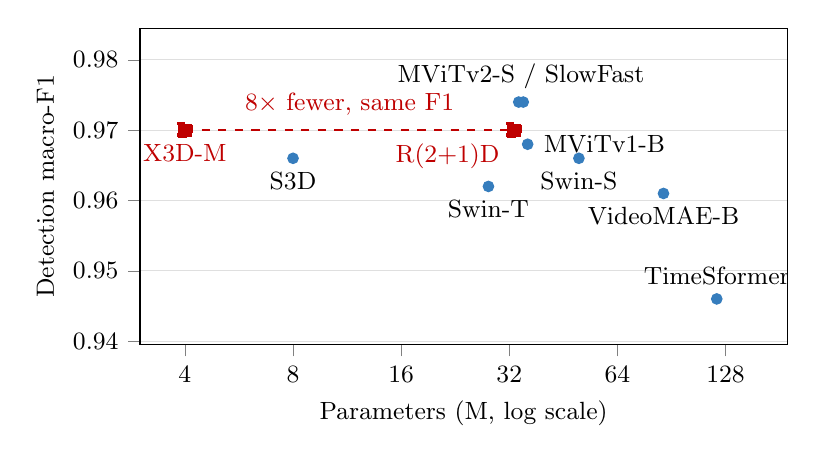
\begin{tikzpicture}
\begin{axis}[
  resultaxis,
  width=9.8cm, height=5.6cm,
  xmode=log, log basis x=2, log ticks with fixed point,
  xlabel={Parameters (M, log scale)}, ylabel={Detection macro-F1},
  xtick={4,8,16,32,64,128},
  xmin=3, xmax=190, ymin=0.9395, ymax=0.9845,
  ytick={0.94,0.95,0.96,0.97,0.98},
  yticklabel style={/pgf/number format/fixed,/pgf/number format/precision=2},
]
\addplot[only marks, wacvblue, mark=*, mark size=1.9pt] coordinates {
  (8,0.966) (28,0.962) (34,0.974) (35,0.974) (36,0.968) (50,0.966) (86,0.961) (121,0.946)};
\addplot[hired, dashed, thick, mark=square*, mark size=2.4pt]
  coordinates {(4,0.970) (33,0.970)};
\node[hired, font=\small, anchor=south]      at (axis cs:11.5,0.9707) {$8\times$ fewer, same F1};
\node[hired, font=\small, anchor=north]      at (axis cs:4,0.9694)    {X3D-M};
\node[hired, font=\small, anchor=north east] at (axis cs:32,0.9694)   {R(2+1)D};
\node[font=\small, anchor=south]      at (axis cs:34.5,0.9745) {MViTv2-S / SlowFast};
\node[font=\small, anchor=north]      at (axis cs:8,0.9654)    {S3D};
\node[font=\small, anchor=north]      at (axis cs:28,0.9614)   {Swin-T};
\node[font=\small, anchor=west]       at (axis cs:37.5,0.968)  {MViTv1-B};
\node[font=\small, anchor=north]      at (axis cs:50,0.9654)   {Swin-S};
\node[font=\small, anchor=north]      at (axis cs:86,0.9604)   {VideoMAE-B};
\node[font=\small, anchor=south]      at (axis cs:121,0.9466)  {TimeSformer};
\end{axis}
\end{tikzpicture}
\end{document}
